% !TEX root = ../thesis_main.tex
\chapter{Theory and state of the art}\label{chap:theory}
This chapter will provide a basis for understanding the principles of this work as well as the phenomena and effects exploited in the later chapters. It will cover the most important aspects, and, of course, for a more detailed description, the cited literature may be consulted. At first, the quantum mechanical approach describing nuclei and spin systems will be given followed by a more application oriented description of the effects occurring and used in NMR and MRI.
    \section{Nuclei and Spins}
        \label{sec:theory:nucleiSpins}
        The postulation of an electron spin in 1926 \cite{uhlenbeck_ersetzung_1925, goudsmit_ontdekking_1971} and later, in 1927, of a proton spin \cite{dennison_note_1927} opened up new areas of research. The discovery opened up numerous new research topics both in basic research, especially in high energy physics, but also in directions leading to applied sciences making use of the spin properties of the nuclei. Nuclear magnetic resonance (NMR, \cite{purcell_resonance_1946-1} ) and Magnetic Resonance Imaging (MRI, \cite{mansfield_medical_1977}) are two sprouts of that development and are the basis of this thesis.
        Each atom or molecule has magnetic properties to which both electrons and the nucleus, i.e. protons and neutrons, contribute. We consider the electrons' contributions to be of a static nature because of their, compared to usual acquisition times, fast movement (Born-Oppenheimer approximation, see \ref{sec:theory:chemicalShift}) and instead turn to the nucleus' magnetic properties. As we want to manipulate nuclei electromagnetically, their magnetic momentum is the relevant physical property in this case.
        The magnetic momentum $\vec M$ of a nucleus is connected to the spin $\vec S$ by the gyromagnetic ratio $\gamma$, a nucleus specific proportionality factor \cite{balanis_advanced_nodate}:
        \begin{equation}
            \vec M = \gamma \vec S
            \label{eq:gyromagneticRatio}
        \end{equation}
        The spin can be described as and mathematically seems to behave like an angular momentum, but is not generated by particle rotation - it is rather an intrinsic property of the particle. Each of the nuclei, in literature and in the following often also simply called "spin", is described by the quantum numbers according to the quantized angular momenta, using quantum numbers j and m.
        The states of the single spin and thus its spin angular momentum can be described fully by the Pauli matrices $\vec{I} = \left\{ \hat{I}_x, \hat{I}_y, \hat{I}_z\right\}$\cite{pauli_zur_1988}
            \begin{align}
                \label{equ:theory:spinStates}
                \vec I^2 \ket{j,m} &= j(j+1)\ket{j,m}\\
                \hat{I}_z \ket{j,m} &= m\ket{j,m}\\
                \hat{I}_\pm \ket{j,m} &= \sqrt{j(j+1)-m(m+1)}\ket{j,m\pm1}
            \end{align}

            where $ \hat{I}_\pm = \hat{I}_x\pm i \hat{I}_y$.

       % We consider the protons and neutrons to be in their spin $\tfrac{1}{2}$ state in all cases considered here, only at very high energies in the \SI{}{\giga\electronvolt}, other states can occur.
        The nucleus then has m~=~(2j~+~1) energy eigenstates that are degenerated at zero magnetic field. If a magnetic field is present though, the energy levels will split with energy differences proportional to the magnetic field strength. The splitting is known as the Zeeman energy splitting.
        \subsection{Zeeman energy splitting}
            If a particle with a spin $S\neq 0$ is exposed to a magnetic field $B_0$, it experiences an energy splitting of its spin-eigenstates due to the fact that different directions of the spins in the magnetic field now have different energies. Both the gyromagnetic ratio and the magnetic field strength determine how big that energy is:
            \begin{equation}
                E_{Z} = -\gamma m B_0
            \end{equation}
            where $E_Z$ is the Zeeman energy of the eigenstate with the magnetic quantum number m.\cite{gerlach_experimentelle_1989, bloch_nuclear_1946}. The negative sign implies that a parallel orientation with the field for particle with positive $\gamma$ is energetically favorable. For example, $^1$H and $^{15}$N, the two main nuclei considered in this work with $\gamma = \SI{42.58}{\\mega\hertz\per\tesla}$ and $\SI{-4.32}{\mega\hertz\per\tesla}$ respectively, show energy splittings into two levels ($2\cdot\tfrac{1}{2}+1$), but of about a factor of 10 stronger for $^1$H due to the by that factor larger gyromagnetic ratio. Additionally, the energetically favorable alignment is different for both nuclei because $^{15}N$ has a negative gyromagnetic ratio (see figure \ref{figure:theory:zeemanSplittings}).
            \begin{figure}
                \centering
                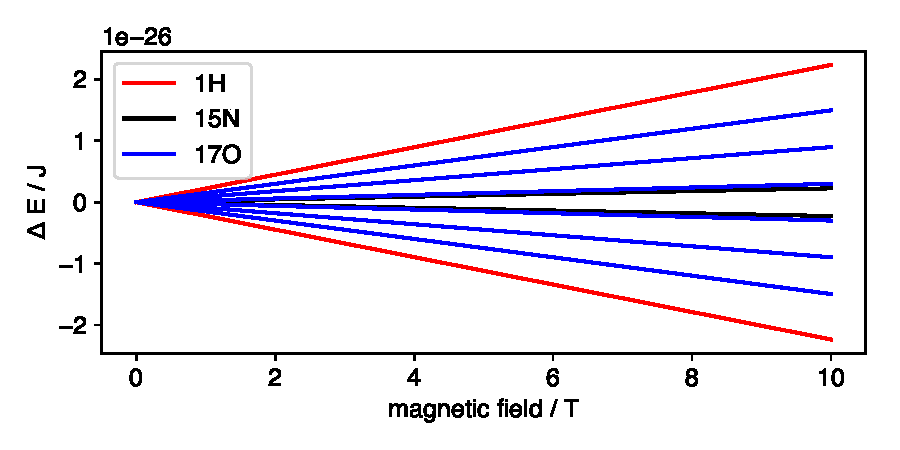
\includegraphics[width=0.9\textwidth]{/figures/theory/zeemanPlot.pdf}
                \caption[Zeeman energy splitting]{The Zeeman energy splittings of three nuclei over magnetic field. Note the difference in slopes for the spin $\tfrac{1}{2}$ nuclei $^1$H and $^{15}$N caused by the different gyromagnetic ratios. Arbitrarily, $^{17}$O, a spin $\tfrac{5}{2}$ nucleus, was plotted to visualize higher order splittings with $2 \cdot\tfrac{5}{2}+1 = 6$ energy levels. }
                \label{figure:theory:zeemanSplittings}
            \end{figure}

            When considering a spin-1/2 particle in a magnetic field along the z-axis (which is the usual choice and does not imply loss of generality), e.g. the proton as a prominent particle in NMR, its spin state can be described by the two eigenstates of $\hat{I}_z$ 
            \begin{equation}
            \ket\alpha = \begin{pmatrix}1\\0\end{pmatrix} \hspace{2 cm} \ket\beta =
            \begin{pmatrix}0\\1\end{pmatrix}
            \end{equation}
            with the eigenvalues of $\pm 1/2$. Using the Pauli matrices to construct the three angular momentum operators
            \begin{align*}
                I_x = \frac{1}{2}
                \begin{pmatrix}
                    0 & 1\\
                    1 & 0
                \end{pmatrix}, 
                I_y = \frac{1}{2}
                \begin{pmatrix}
                    0 & -i\\
                    i & 0
                \end{pmatrix}, 
                I_z = \frac{1}{2}
                \begin{pmatrix}
                    1 & 0\\
                    0 & -1
                \end{pmatrix} 
            \end{align*}
            and the corresponding shift operators $I_\pm = \frac{1}{2} \hat 1 \pm I_z$ equations \ref{equ:theory:spinStates}ff can be expressed as:
            \begin{align*}
                \vec I^2 \ket{\alpha} &= \frac{1}{2}\ket{\alpha}&\vec I^2 \ket{\beta} &= \frac{1}{2}\ket{\beta}\\
                \hat{I}_z\ket\alpha &= \frac{1}{2}\ket\alpha &\hat{I}_z\ket\beta &= -\frac{1}{2}\ket\beta\\
                \hat{I}_+\ket\alpha &= 0 &\hat{I}_+\ket\beta &= \ket\alpha\\
                \hat{I}_-\ket\alpha &= \ket\beta& \hat{I}_-\ket\beta &= 0
            \end{align*}
            Generally, every spin-1/2 particle can be in any superposition of those two eigenstates:
            \begin{equation}
                \ket\psi = c_\alpha \ket\alpha + c_\beta \ket \beta = \begin{pmatrix} c_\alpha \\
                c_\beta\end{pmatrix}
            \end{equation}
            These superposition states in general evolve under the spin Hamiltonian of the system.  To do so, usually the density matrix formalism is introduced.
             In this case, the
            expectation value of an operator for a single spin $\braket{\hat Q}$ is given by 
            \begin{equation}
            \bra\psi\hat Q\ket\psi = \left( c_\alpha^*, c_\beta^*\right)
            \begin{pmatrix}
                Q_{\alpha\alpha} Q_{\alpha\beta}\\
                Q_{\beta\alpha} Q_{\beta\beta}
            \end{pmatrix}
            \begin{pmatrix}
                c_\alpha\\
                c_\beta
            \end{pmatrix}
            \end{equation}
            as described in \cite{sakurai_modern_2017}. This is equal to the trace of the density operator
            $\ket\psi\bra\psi$ multiplied with said operator \cite{levitt_spin_nodate}
            \begin{equation}
                \braket{\hat Q} = \Tr \left\{\ket\psi\bra\psi\hat Q\right\}
            \end{equation}
            As a sample in our case does not consist of one, but many nuclei (\SI{1}{\milli\liter} of water consists of $\sim$ $7\cdot 10^{22}$ spins), the evolution of all of those spins needs to be considered to describe the system. 
            It follows that the expectation value of an observable becomes the sum of their individual statistically weighted expectation values:
            \begin{equation}
                \hat Q_{ensemble}= \bra{\psi_1}\hat Q\ket{\psi_1} + \bra{\psi_2}\hat Q\ket{\psi_2} + \hdots =
                \Tr{\left\{\left(\ket{\psi_1}\bra{\psi_1} + \ket{\psi_2}\bra{\psi_2}+ \hdots \right) \hat Q\right\}}
            \end{equation}
            The first part of the trace's argument is closely related to the density matrix which corresponds to the average sum of the individual density operators:
            \begin{equation}
                \hat\rho = \overline{\ket\psi\bra\psi} = \frac{1}{N} (\ket{\psi_1}\bra{\psi_1} + \ket{\psi_2}\bra{\psi_2} + \dots).
            \end{equation}
            For a large number of spins, the macroscopically observable value Q is then
            \begin{equation}
                Q_{macro} = \left< Q \right> = N \Tr \left( \hat{\rho} \hat{Q}\right)
            \end{equation}
            For a spin-1/2 ensemble, the density matrix in thermal equilibrium is
            \begin{equation}
                \hat \rho = \begin{pmatrix} \frac{1}{2}+\frac{1}{4}\mathbb{B}& 0\\ 0&
                \frac{1}{2}-\frac{1}{4}\mathbb{B}\end{pmatrix} = \frac {1}{2} \hat1 + \frac{1}{2} \mathbb{B}
                \hat I_z
            \end{equation}
            with $\mathbb{B} = \frac{\hbar\gamma B_0}{k_b T}$. That means that in thermal equilibrium, the non-diagonal elements (so-called coherences) are zero, while there is a slight overpopulation (see section \ref{sec:theory:HP}) of one of the two states at non vanishing magnetic fields. Through deflection from that equilibrium, coherences are populated as described in the following section.
        \subsection{Radiofrequency pulses}
        \label{sec:theory:RFPulses}
            Using the density matrix formalism, the effect of radiofrequency pulses is described by rotational operators that can be
            applied to the whole ensemble. A pulse $\hat R_\phi(\beta)$ of phase $\phi$ (corresponding
            to the axis around which magnetization is rotated) and angle $\beta$ where
            $\beta=\omega_{nut} \cdot \tau_p$ acting on a state $\ket\psi$ is described by 
            \begin{equation}
                \ket{\psi_\tau}= \hat R_\phi(\beta)\ket\psi
            \end{equation}
            Calculating the density matrix now leads to
            \begin{equation}
                \hat {\rho_\tau} = \overline{\ket{\psi_\tau}\bra{\psi_\tau}} = \overline{\hat
                    R_{\phi}(\beta)\ket\psi\bra\psi \hat R_\phi(-\beta)}
            \end{equation}
            where the overbar describes the averaging over all spins in the ensemble \cite{popov_modern_1990, chizhik_magnetic_2014} Finally, as we are considering the rotation to be the same for every single spin in the ensemble, the formula can be reduced to
            \begin{equation}
                \hat\rho_\tau = \hat R_\phi(\beta) \hat \rho \hat R_\phi(-\beta)
            \end{equation}
            where $\rho$ is the average density matrix of the ensemble meaning a rotation of the magnetization corresponds to a rotation of the density matrix. If, e.g., we consider a $\SI{90}{\degree}$ pulse around the x-axis on the previously described equilibrium for a spin-1/2 ensemble it follows \cite{hosur_scaling_1990, levitt_spin_nodate}:
            \begin{equation}
                \begin{split}
                    \hat\rho_\tau = \hat R_x(\pi/2)\hat\rho\hat R_x(-\pi/2) &= \frac{1}{2} \hat 1 +
                    \frac{1}{2} \mathbb{B}\hat R_x(\pi/2) \hat I_z \hat R_x(-\pi/2)\\
                    &=
                    \begin{pmatrix}
                        \frac{1}{2} & -\frac{1}{4i}\mathbb{B}\\
                        \frac{1}{4i}\mathbb{B}\ & \frac{1}{2}
                    \end{pmatrix}
                \end{split}
            \end{equation}
            It can be equally shown that a $\SI{180}{\degree}$ pulse inverts the populations of the diagonal elements while the coherences are untouched.  If the system is not in thermal equilibrium, the density matrix will evolve and generally relax back to its equilibrium state. If one neglects said relaxation at first, the free evolution can be described by
            \begin{equation}
                \begin{split}
                    \ket\psi_\upsilon &= \hat R_z(\Omega^0\upsilon)\ket\psi_\tau ~ \mathrm{and} \\
                    \hat\rho_\upsilon &= \hat R_z(\Omega^0\upsilon)\hat\rho_\tau\hat R_z(-\Omega^0\upsilon)
                \end{split}
            \end{equation}
            where $\upsilon$ is the free evolution time and $\Omega_0$ is the frequency offset off the central, rotating frame frequency. Only a time dependent phase $\exp{(\Omega^0 \upsilon)}$ is added to the coherences that way and the populations stay constant. This confirms the macroscopic observation that the ensemble of spins behaves like a rotating vector of magnetization in the x-y-plane (w\textbackslash o relaxation). If relaxation is added to the scheme as a phenomenological effect, we can differentiate between relaxation of the coherences ($T_2$ relaxation) and that of the states ($T_1$ relaxation). The former affects the non diagonal elements only which will decay to zero over time while the latter brings the populations of the states back to thermal equilibrium. That can be expressed by
            \begin{equation}
                \rho_{ij, \upsilon} = \rho_{ij, \tau} \exp{((\pm i\Omega^0-\lambda)\upsilon)},~\mathrm{i,j~=~ 1,2(+)~or~2,1(-)}
            \end{equation}
            for the non diagonal elements where $\upsilon = T_2^{-1}$ and
            \begin{equation}
                \rho_{ii,\upsilon} = (\rho_{ii,\tau} - \rho_{ii}^{eq})\exp(-\upsilon/T_1)+\rho_{ii}^{eq}
            \end{equation}
            for the diagonal elements \cite{levitt_spin_nodate}.
        \subsubsection{Free time evolution}
        States that are not eigenstates of the system will evolve over time. If relaxation and external influences such as pulses or gradients are zero, the time evolution of the density matrix and thus the states is described by \cite{sakurai_modern_2017, levitt_spin_nodate}:
        \begin{equation}
            \frac{d}{dt} \sigma(t) = -i \left[\mathcal{H}, \sigma(t)\right]
        \end{equation}
        which, because of the time independent Hamiltonian is solved by a simple exponential propagator:
        \begin{equation*}
            U(t-t_0) = \exp(-i\mathcal{H}(t-t_0))
        \end{equation*}
        The density matrix at time t thus reads:
        \begin{equation}
            \sigma(t-t_0) = U(t-t_0) \sigma(t_0) U^\dagger(t-t_0).
        \end{equation}
        \subsubsection{Signal detection}
        The signal induced into the receive coil of a scanner (sec. \ref{sec:matMeth:rfPulses}, \ref{sec:matMeth:receiveCoil} for hardware details) is described by the expectation value of the $\hat{I}_+ = \hat{I}_x + i\hat{I}_y$ operator \cite{levitt_spin_nodate}:
        \begin{equation}
            S(t) = \left< \hat{I}_x + i\hat{I}_y \right> = tr\left(\sigma(t)\hat{I}_x + i\hat{I}_y\right)
        \end{equation}
        In addition to the pure signal, there will also be a contribution of noise to the overall signal. This contribution will be arbitrarily distributed and increases with the root of the number of acquisitions: $S_{noise} \propto \sqrt{n}$. The NMR signal increases linearly with the acquisitions $S_{NMR} \propto n$. The combined signal to noise ratio thus increases with
        \begin{equation}
            SNR =  \frac{S_{NMR}}{ S_{noise}}  \propto \frac{n}{\sqrt{n}} = \sqrt{n}
        \end{equation}
        This is why decent noise suppression and use of low noise materials to build coils and readout electronics are key to keep measurement times small (i.e. to reduce the necessity of averaging to reach acceptable SNR values).
        where $\sigma(t_0)$ is the density matrix at time $t_0$.
        \subsection{Multiple spin ensembles}
            The description above was all formulated for an ensemble of isolated spins. It can - and has to - be extended to describe more complex systems of molecules containing multiple, interacting spins. To do so, the product operators, product states and product density matrices of all operators and states need to be calculated. This can be done by expanding the operators of the single spin system into the direct product space describing a N spin system:
            \begin{equation*}
                A^p_n = \mathbb{I}_0\otimes\mathbb{I}_1\cdots \mathbb{I}_{n-1} \otimes A_n \otimes \mathbb{I}_{n+1}\cdots \mathbb{I}_N
            \end{equation*}
            where $\mathbb{I}_i$ is the unity matrix of operator $A_i$. The product operators have the advantage of making normal matrix multiplications possible where otherwise, Kronecker products were needed \cite{green_theory_2012-1}:
            \begin{equation}
                A_n\otimes A_m = (A_n \otimes \mathbb{I}_m)(\mathbb{I}_n \otimes A_m) = A^p_nA^p_m
            \end{equation}
            Note that this is an especially convenient notation but will also cover coupling effects between the different species in the off-block-diagonal elements. Similarly, the extended states are established as Kronecker products of their single states:
            \begin{equation}
                \ket{a_1,a_2, \dots, a_N} = \ket{a_1}\otimes\ket{a_2}\otimes\dots\otimes\ket{a_N}
            \end{equation}
            with all N substates and their respective quantum numbers. This leads to a product state vector with all substates written below each other as the initial states are only vectors, not matrices. Additionally, as we want to describe a ensemble of spins, the density matrix is constructed in product space:
            \begin{equation}
                \sigma^p = \sigma_1 \otimes\sigma_2\dots\otimes\sigma_N
            \end{equation}
        \subsection{Hamiltonian and couplings}
            To describe the energies of a spin ensemble, the Hamiltonian is constructed
            \begin{equation*}
                \mathcal{H}\ket{a_n} = E_n \ket{a_n}.
            \end{equation*}
            For the magnetic Hamiltonian, equation \ref{eq:gyromagneticRatio} is used with the angular momentum operator $\vec{\hat I_n} = I_{nx}\hat{e}_x + I_{ny}\hat{e}_y + I_{nz} \hat{e}_z$
            \begin{equation}
                \mathcal{\hat H} = - \vec{\hat M}_n \vec B
            \end{equation}
            were $\vec{\hat M}_n $ is the magnetic moment of the nth nucleus. This equation simplifies if we consider the static magnetic field to be in z-direction only, without loss of generality \cite{ashok_lectures_2013}:
            \begin{equation}
                \label{equation:theory:staticFieldHamiltonian}
                \mathcal{\hat H}_n^{stat} = - \gamma_n B_0 \hat{I}_{nz}
            \end{equation}
            Equation \ref{equation:theory:staticFieldHamiltonian} is the basis of the Larmor frequency $\omega = \gamma B_0$ calculations described in section \ref{sec:theory:larmorFrequency}.
            In addition to the main magnetic field $B_0$, other effects influence the overall energy of the nuclei. These are intra- and inter-molecular dipole-dipole couplings and quadrupole couplings, intra-molecular J-coupling and spin rotation and so-called chemical shift, a interaction or shielding effect of electrons towards the nuclei.
            In NMR of liquids, the strongest contribution usually is the chemical shift delivering the largest contribution. 
        \subsubsection{Chemical shift}
        \label{sec:theory:chemicalShift}
            The chemical shift can be considered linearly dependent on the external magnetic field meaning that for the chemical shift induced field $B_n^{cs}$ of the nth nucleus
            \begin{equation}
                \vec B_n^{cs} = \boldsymbol\delta_n \vec B_0
            \end{equation}
            resulting in a corresponding Hamiltonian term if we consider the chemical shift to be isotropic (i.e. we consider the chemical shift tensor to have three equal diagonal entries only \cite{levitt_spin_nodate}) and additionally constraining the principal magnetic field to the z direction, we get:
            \begin{equation}
                \mathcal H_n^{cs} = -\gamma \delta_n B_0 \vec I_{nz}
            \end{equation}
            where $\delta_n$ is the average over all angles of the chemical shift tensors z component, which in isotropic liquids is constant $\delta_n = \overline{ \boldsymbol\delta_{zz}(\Theta)}$ \cite{abraham_proton_1997}.
        \subsubsection{Spin-Spin- and J-couplings}
            The direct spin-spin couplings between different nuclei also known as dipolar couplings average out in the Hamiltonian in case of liquid state NMR due to rapid molecular motion compared to the timescales of the Zeeman interaction. Different couplings are still observable in the recorded NMR spectra. These are indirect couplings or J-couplings transduced through the electrons. The Hamiltonian of this interaction is described by the coupling tensor, $J_{nm}$ and the corresponding angular momentum operators
            \begin{equation}
                \mathcal{H}^J_{nm} = \hat{\vec I}_n \vec J_{nm} \hat{\vec I}_m
            \end{equation}
            As for the chemical shift before, this can be simplified for isotropic liquids where the tensor can be reduced to a scalar coupling constant. The J coupling is independent of the magnetic field applied, i.e. the line splittings in the spectra are of the same size when magnetic field changes. The overall spin Hamiltonian then reads:
            \begin{equation}
                \mathcal{H}^0 = \omega_1\hat{I}_{1z} + \omega_2\hat{I}_{2z} + 2\pi J_{12}\hat{I}_1\hat{I}_2 + d_{12}(3\hat{I}_{1z}\hat{I}_{2z} - \hat{I}_1\hat{I}_2)
            \end{equation}
            with the individual Larmor frequencies $\omega_i$ and the J- and dipole-dipole coupling terms $J_{12}$ and $d_{12}$.
            By substituting the shift operators in the equation and dropping the dipole-dipole term before setting $\omega_{12} = \pi J_{12}$, the overall spin Hamiltonian reads:
            \begin{equation}
                \mathcal{H}^0 = \frac{1}{2}
                \begin{pmatrix}
                    \omega_1+\omega_2+\omega_{12} & 0 & 0 & 0\\
                    0 & \omega_1-\omega_2-\omega_{12} & 2\omega_{12} & 0 \\
                    0 & 2\omega_{12} & -\omega_1+\omega_2-\omega_{12} & 0\\
                    0 & 0 & 0 & -\omega_1-\omega_2+\omega_{12}
                \end{pmatrix}
            \end{equation}
            Usually, two cases are differentiated, the weak and the strong coupling regime. Strong coupling, is observed when the J-coupling is in the order of the nucleis' Larmor frequency differences, i.e. $\Delta \nu / J \approx 1$. The extreme case of no chemical shift difference, i.e. $\omega_1 = \omega_2=\omega$ is called magnetic equivalence.
            The latter can be described by a new set of eigenstates that diagonalize the Hamiltonian:
            \begin{equation}
                \mathcal{H}^0 = \frac{1}{2}
                \begin{pmatrix}
                    \omega_0+ \tfrac{\pi}{2} J_{12} & 0 & 0 & 0\\
                    0 &  \tfrac{\pi}{2}J_{12} & 0 & 0 \\
                    0 & 0 & -\omega_0 + \tfrac{\pi}{2}J_{12} & 0\\
                    0 & 0 & 0 & -\tfrac{3\pi}{2}
                \end{pmatrix}
            \end{equation}
            The Hamiltonians eigentstates form a triplet and a singlet where the triplet state's energies are shifted by $2\pi J_{12}$ from the singlet's energy. The outer triplet states are additionally shifted by $\pm\omega_0$ from the central triplet state, i.e. by the uncoupled Zeeman shift.
            As the energy difference is equally large (because of the assumption that isotropic liquids' spin-spin coupling averages out, otherwise, additional $D_{12}$ would have to be considered), only a single line can be observed in the NMR spectrum.
            Weak coupling, on the other hand, means that the J coupling is small compared to the chemical shift differences:
            \begin{equation*}
                \frac{\delta\nu}{J} >> 1 \rightarrow \frac{1}{2} |\omega_{12}| << |\omega_1-\omega_2|
            \end{equation*}
            meaning a weakly coupled regime may be considered when half the J-coupling is much smaller than the chemical shift difference. The Hamiltonian of the system can be constructed in the secular approximation where all off-diagonal elements have to be small compared to the difference of their diagonal partners: $\mathcal{H}_{nm} << \mathcal{H}_{nn} - \mathcal{H}_{mm}$ which corresponds to the definition of weak coupling \cite{levitt_spin_nodate}.
            In this case, the Hamiltonian reads
            \begin{equation}
                \mathcal{H} = \omega_1\hat{I}_{1z} + \omega_2\hat{I}_{2z} + \omega_{12}2\hat{I}_{1z}\hat{I}_{2z}
            \end{equation}
            with the eigenenergies
            \begin{align}
                E_{\alpha\alpha} =& \tfrac{1}{2} ( \omega_1 + \omega_2 + \omega_{12})\\
                E_{\alpha\beta}  =& \tfrac{1}{2} ( \omega_1 - \omega_2 - \omega_{12})\\
                E_{\beta\alpha}  =& \tfrac{1}{2} (-\omega_1 + \omega_2 - \omega_{12})\\
                E_{\alpha\alpha} =& \tfrac{1}{2} (-\omega_1 - \omega_2 + \omega_{12})
            \end{align}
            The additional J coupling breaks the double degeneracy of the central energy level of the pure Zeeman states by shifting them by $\omega_{12} = 2\pi J_{12}$. The resulting spectrum thus shows four instead of the previous two peaks.
            %coupling between nuclei of the same kind (homonuclear coupling) and that of nuclei of different kinds (heteronuclear coupling) \cite{levitt_spin_nodate}.
            %\begin{equation}
            %    H_{nm} = 2\pi J_{nm} \vec{\hat{I_n}} \vec{\hat{I_m}} (heteronuclear case)
            %\end{equation}
            %\begin{equation}
            %    H_{nm} = 2\pi J_{nm} \vec{\hat{I_n}} \vec{\hat{I_m}} (heteronuclear case)
            %\end{equation}
            %\todo{correct boldness, weird latex bahavior}
            %The coupling constant $J_nm$ is calculated using the gyromagnetic ratios of the nuclei, in case of hydrogen usually 
            %\begin{equation}
            %    J_{HH} = \gamma_H \gamma_H A
            %\end{equation}
            %is used to estimate the coupling, where $A$ is calculated through known electron densities and nucleus distances.
            %For other nuclei such as $^{15}N$ or $^{13}C$, the coupling that is calcuated for $^1H$ can be reused \cite{levitt_spin_nodate}:
            %\begin{equation}
            %J_{HX} = J_{HH} \frac{\gamma_X}{\gamma_H} \mathrm{and} J_{XX} = J_{HH} \left(\frac{\gamma_X}{\gamma_H} \right)^2
            %\end{equation}
            %Knowing all relevantly contributing effects, the overall hamiltonian can be constructed. This can be done in the laboratory frame
            %\begin{align}
            %    \mathcal{H} &= \sum_n\left(\mathcal{H}_n^z + \mathcal{H}_n^J/2\right)\\
            %                &= \sum_{n}\omega_N\hat{I}_{nz} + \sum_{n<m}2\pi J_{ij} \hat{\mathbf{I}}_n\hat{\mathbf{I}}_m
            %\end{align}
            %or the rotating frame where the center frequency $\omega_{ref}$ is zero, i.e. frequencies relative to the center frequency are considered:
            %\begin{equation}
            %    \mathcal{H} = \sum_n{\Omega_n\hat{\mathbf{I}}_{nz}} + \sum_{n<m}{2\pi J_{nm}\hat{mathbf{I_n}}\hat{\mathbf{I_m}}}
            %\end{equation}
            %with $\Omega_i = \omega_i - \omega_{ref}$ in the rotating frame of reference.
            %\cite{macomber_complete_1997}
            %If the coupling is weak compared to the energy difference of the states, i.e. $\Delta E >> J_{nm}$, the secular approximation can be considered valid. \todo{check sentence}
    \section{NMR}
    Nuclear Magnetic Resonance (NMR) is a technique that emerged in 1946 with the discovery of the absorption properties of nuclei irradiated with electromagnetic waves resonant to their Larmor frequencies \cite{purcell_resonance_1946-1}. The subsequent observation of signal from those previously excited nuclei \cite{rabi_space_1937,bloch_nuclear_1946}, later mostly known as free induction decay (FID) paved the road to the now well established method which in the beginning was primarily used in chemistry for structural analysis of molecules and chemical kinetics \cite{perrin_application_1990,lipkind_computer-assisted_1988}. This chapter will describe the theoretical basis of that technique keeping in mind that many theoretical aspects are already covered in section \ref{sec:theory:nucleiSpins} and will only be mentioned briefly. 
        \subsection{Larmor frequency}
        \label{sec:theory:larmorFrequency}
            Inside an external magnetic field $B_0$, a magnetic dipole $\mu$ will precess with a frequency
            proportional to $B_0\cdot \mu$. This also applies to  particles with a spin $S\neq0$ and thus
            a magnetic moment $\mu\neq0$. The precession is a result of the torque $\mu\times\vec B$
            exerted on the magnetic dipole moment with the frequency
            \begin{equation}
                f_L=\frac{\omega}{2\pi} = \frac{\gamma}{2\pi}\cdot B
            \end{equation}
        \subsection{Free induction decay}
        The NMR signal induced in a resonant circuit after a \SI{90}{\degree} pulse is called free induction decay (FID). It is generated by the net magnetization of the sample precessing in the static magnetic field B0 with its Larmor frequency $\omega_0$. The current induced in the receive coil is stored in the resonant circuit with the resonance frequency tuned to the sample's Larmor frequency. The decay in the name describes the reduction of the signal due to relaxation of the nuclei towards thermal equilibrium, see section \ref{chapter:theory:relaxation}.
        \subsection{Fourier transform, signal and signal to noise}
        \label{chapter:theory:fourierTransform}
        To analyze the acquired FIDs and echos, they're usually Fourier transformed leading to a frequency analysis of the signal. This is achieved using the well known formula \cite{farrar_pulse_2012}
            \begin{equation}
                F(\omega) = \int^{\infty}_{-\infty}S(t) \exp(-i\omega t)dt
            \end{equation}
            As the Fourier transform's input is complex, the signal is expanded to a complex form by comparison to a carrier frequency and splitting the signal into a real, in phase and an imaginary, \SI{90}{\degree} phase shifted part.
            Note that the signal received is usually mixed with the center frequency of the NMR machine as the carrier frequency leading to the rotating frame frequencies being observed in the FID or echo. The frequency axis can subsequently be shifted to provide absolute frequencies again, but mostly is displayed as the relative deviation off a central frequency defined by the user or a reference sample.
            The signal consists of both the pure signal and additional noise from different sources. These include thermal noise, environmental noise and different forms of intrinsic electronics noise \cite{noauthor_henry_nodate}.
            If a signal is low compared to noise levels, signal averaging can be applied to improve SNR. As signal increases with the number of scans n while noise does so only with $\sqrt n$ due to its random direction, n averages will improve the SNR by $n/\sqrt{n} = \sqrt{n}$ if other factors stay unchanged \cite{edelstein_intrinsic_1986}.
            In the spectrum, one relaxation time, $T_2^*$ can be directly calculated as the inverse of the linewidth at half maximum for a specific nucleus. That means that a long $T_2^*$ leads to a high spectral resolution, making shimming an important prerequisite in NMR.
        \subsection{Chemical shift}
            The Larmor frequency of nuclei in NMR is largely governed by $B_0$ and $\mu$, but other factors do influence it on a more subtle scale. The most prominent effect besides the Zeeman splittings is the chemical shift which originates in the shielding of $B_0$ by the electrons' magnetic dipoles surrounding the nucleus or molecule and is visible in the spectra \cite{gottlieb_nmr_1997}. The shielding thus generally leads to a shift of precession frequency. The chemical shift is calculated as the relative frequency quota towards another known sample's reference frequency:
            \begin{equation}
                \delta = \frac{\nu_{sample} - \nu_{reference}}{\nu_{reference}}
            \end{equation}
            To have a field independent value for the chemically shifted frequency (same goes for other couplings), which, to a good approximation, scales linearly with the field, it is usually expressed in ppm of the center frequency. That way, the linear dependence on the field is canceled by division through said field and a field independent value emerges.
        \subsection{J-coupling}
        In addition to the change in the field by the electrons dipoles, the nucleis' magnetic dipoles inside a molecule will also interact. The interaction can be conveyed either directly or via the electrons' spins. The direct interaction is neglectable in liquids due to fast rotating molecules that average this interaction's sum to zero. The indirect interaction via the electrons can, however, lead to a frequency shift resulting in multiplets usually on scales smaller than the chemical shifts, i.e. in the $\SI{}{\hertz}$ range.
        J-couplings can be measured by evaluating the distance of peaks in 1-D spectra, or, if resolution does no suffice, through the evolution of nuclei phases under the coupling using 2d-NMR spectra (see \ref{chapter:theory:2DNMR} and \cite{ottiger_measurement_1998}).
        \subsection{Flip angle}
        An external, on-resonant magnetic field will, as described in section \ref{sec:theory:RFPulses}, cause the magnetization of an ensemble of spins to flip by an angle $\alpha$ known as the flip angle (FA). A FA of $\mathrm n\cdot 180 \deg + 90 \deg$ with $n \in \mathbb{N}$ will rotate the magnetization to the transverse plane perpendicular to the magnetic field resulting in an FID. Pulses of $\mathrm n\cdot 180 \deg$ will keep the magnetization aligned with the magnetic field axis or invert it, therefore not resulting in a FID or echo. All other FAs will produce a linear combination of the two cases. Note that in case of a \SI{180}{\degree} pulse, relaxation occurs along the z-axis despite the lack of a NMR signal. The FA is defined as the time integral over the coil voltage with a coil specific calibration factor $A_c$:
            \begin{equation}
                FA = A_c \int_{t=0}^{T_p}{V(t)dt}
            \end{equation}
            This means that, if the coil has been calibrated for one pulse form, e.g. a simple box pulse 
            \begin{equation}
                V(t) = A\sin{\omega_{RF} t + \phi_0} u(t)u(t-T_{RF})
            \end{equation}
            with duration $T_{RF}$ and Heaviside function $u(t)$, every other pulse's FAs with arbitrarily shaped amplitude $A(t)$ can be calculated from that. This of course excludes effects like relaxation during pulsing \cite{wang_factors_2006}, which can be relevant especially for long pulses and is also not considering hardware limitations on the coils concerning maximum voltage or wattage.
        \subsection{Shimming}
        As the magnetic field is generated by a superconductor (compare section \ref{sec:theory:superconductor}) will not be perfectly homogeneous by itself and samples inside the magnet introduce changes in the magnetic susceptibility that further disturbs the magnetic field, shimming, i.e. the retrospective homogenization of the field, plays an important role in NMR and MRI. Different order shims are differentiated, referring to the order of the polynomial they resemble e.g. for a linear shim in x direction
            \begin{equation}
                B(x) = B_0 + B_{sh} * x.
            \end{equation}
            where $B_{sh}$ is the desired magnetic field per unit of length.
            Additionally, magnetic field gradients, usually also linear (often even using the exact same hardware) are used for spatial encoding in MRI applications \ref{sec:theory:magneticGradient}.
        \subsection{A simple NMR experiment}
        The most basic experiment in NMR is the exposure of a spin ensemble to a $\SI{90}{\degree}$ RF pulse and subsequent readout. This will convert the longitudinal magnetization to transversal magnetization $\SI{90}{\degree}$ which precesses around the z axis with its Larmor frequency $\omega_L$ afterwards. Using a coil\ref{sec:matMeth:rfPulses} mounted around the sample, the alternating field caused by the rotating magnetization will induce a current driving the resonant circuit (eq. \ref{equation:theory:maxwell}). That signal - FID or echo - can be recorded as the voltage over the resonant circuit. It can be described by a dampened sine wave
            \begin{equation}
                S(t) = S_0 \exp(i(\omega - \omega_0)  t + \phi) \exp(-\tfrac{t}{T_2^*})
            \end{equation}
            where $\omega$ is the Larmor frequency of the observed particle, $\omega_0$ is the center frequency of the system and $T_2^*$ is the effective dephasing time constant (see \ref{chapter:theory:relaxation}). The phase $\phi$ varies depending on the axis of rotation chosen for the pulse. Mostly, x- or y-pulses are used rotating the magnetization around the respective axis and resulting in phase shifts of \SI{90}{\degree} (x, y, -x, -y). As described in the NMR section (\ref{chapter:theory:fourierTransform}), the signal can then be Fourier transformed and will give insight into the local environments of the nuclei, i.e. their chemical shifts, the couplings they experience and also their relaxation rates (if experiments are repeated with different timings). 
        \subsection{Relaxation}
        \label{chapter:theory:relaxation}
        In addition to the free time evolution of the states, the longitudinal magnetization will decay back to thermal equilibrium after being deflected from it. Two relaxation mechanisms are differentiated: spin-lattice and spin-spin relaxation. The first process, spin-lattice relaxation, is also called T$_1$ relaxation and is an exponential decay (figure \ref{theory:figure:relaxation}, middle). The second mechanism, responsible for the decay of the transverse magnetization has time constant called $T_2$ (figure \ref{theory:figure:relaxation}, left) that is usually much smaller than T$_1$ \cite{levitt_spin_nodate}. $T_2$ relaxation occurs because of different magnetic fields experienced by the individual spins leading to a dephasing of the signal. That can be due randomly modulated spin interactions ($T_2$) and also due to magnetic field inhomogeneities ($T_2i$). Both effects are combined are described by the effective relaxation constant $T_2^*$ \cite{chavhan_principles_2009}.
            \begin{figure}
                \centering
                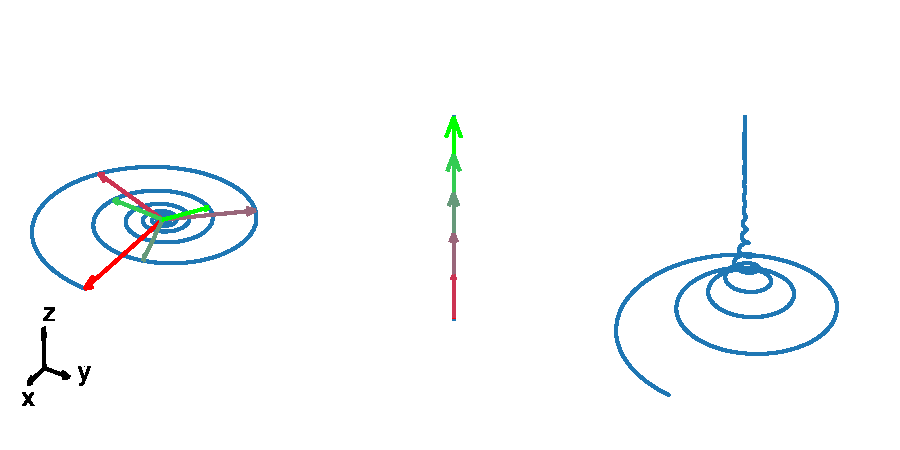
\includegraphics[width=0.9\textwidth]{/figures/theory/relaxation.pdf}
                \caption[Relaxation in NMR]{Exemplary plots of the T$_1$ and $T_2^*$ relaxation after a \SI{90}{\degree} FA shown via the magnetization and its temporal development. On the left, the magnetization in the xy-plane is shown with six arrows indicating equal time-steps. In the center, equal time-steps for the z-magnetization are shown. On the right, both cases are combined to show the overall magnetization. Note that generally, T$_1$ is larger than $T_2$ (here a factor of 40 difference).}
                \label{theory:figure:relaxation}
            \end{figure}
         The main contribution to T$_1$ relaxation arises from dipolar couplings \cite{levitt_spin_nodate}, i.e. couplings between the nuclei in solution and microscopic field changes in magnitude and direction due to other nuclei and electrons fields they move through because of molecular motion. These slight changes interfere with the otherwise uniform precession of the spins around the magnetic field. That way, every spin precesses on slightly different axes shifted from the external field axis and will, on average, align (or anti-align, depending on $\gamma$) with the magnetic field with a slightly higher probability. The timescales of molecular motion are longer than those of spin precession by many orders of magnitude (\si{\mega\hertz} to \si{\hertz}) and the additional fields are small compared to the static magnetic field. Over long timescales, the small anisotropies add up to cause the spin-lattice relaxation. The solution to the phenomenological description of the relaxation, i.e. the  evolution of its magnetization is easily derived:
        \begin{equation}
            M_L(t) = M_0(1 - \exp{-t/T1})
        \end{equation}
        Spin-spin relaxation or transversal relaxation is a usually faster process that describes the dephasing of the single nuclei's spins by exposure to different magnetic field strengths. Macroscopically, the equation
        \begin{equation}
        \frac{dM_{x,y}}{dt} = - \frac{M_{x,y}}{T_2}
        \end{equation}
        is solved, a mono-exponential signal decay described by its time constant $T_2$:
        \begin{equation}
            M_T(t) = M_0\exp{\left(\frac{-t}{T_2}\right)}
        \end{equation}
        The parameters are mostly derived experimentally, but can also be theoretically estimated \cite{kaupp_calculation_2003}.
        \subsection{Inversion recovery and spin echos}
            T$_1$ times of a sample can be measured using inversion recovery experiments. This is usually implemented by a \SI{180}{\degree} pulse followed by \SI{90}{\degree} pulses separated by different evolution times $T_{ev}$. Alternatively, the \SI{90}{\degree} angle can be replaced by many, smaller flip angle pulses. That will make acquisition faster, but has to be considered in the interpretation of the data. For non-uniform samples where the relaxation constants differ over the sample distribution,, T$_1$ values can also be acquired with a spatial encoding using steady state sequences \cite{scheffler_t1_2001}.
            The dephasing of the signal can be fast, but a part of the magnetization, defined by the difference between the T$_2$ and T2* relaxation constants (i.e. between the respective processes), can be regained through refocusing of the magnetization. The inversion can be induced by a \SI{180}{\degree} RF pulse, in steady state measurements, often smaller pulses are used. The "resurrected" signal is called "echo", the time between multiple echoes is called the echo time TE. Multiple echos can be recorded if multiple inversion pulses are applied, but different effects effectively reduce the signal in the course of the recording:
            \begin{itemize}
                \item Diffusion and convection will reduce the efficiency of the signal recovery because both external fields and coupling environments may change due to the change in position.
                \item Pure $T_2$ decay is not recoverable and will reduce the signal.
                \item T$_1$ relaxation reduces the overall transversal magnetization and thus the signal amplitude exponentially.
            \end{itemize}
             These effects can be brought to a steady state equilibrium, meaning that between two consecutive readouts, the same relaxation occurs. Therefore, steady state sequences are the tool of choice for imaging where nucleus density or differences in T$_1$ or $T_2$ shall be observed  \cite{nitz_contrast_1999}.
        \subsection{2D-NMR}
        \label{chapter:theory:2DNMR}
        In addition to the standard NMR spectrum that can get difficult to interpret when many or large molecules are present and multiple nuclei contribute to the signal, a 2D NMR method called COSY emerged in 1976, the simplest and most widely used 2DNMR method on which many other sequences are based  \cite{spie_ad_1982-1}. As the name suggests, spectra are not recorded and shown in the usual 1D-plot, but in a 2D plot providing an additional dimension to display more information. The method is very similar to the MRI method described in chapter \ref{sec:theory:MRI} although here, no field gradients are necessary yet: the second dimension simply shows the development of certain nuclei's signals under a specific interaction during a varying evolution time that is defined by the pulse sequence. By varying the evolution times and Fourier transforming the spectra in the second spatial dimension, the frequency of that interaction will be indicated \cite{finster_two-dimensional_1980}.
        \subsection{Field Gradients}
            \label{sec:theory:magneticGradient}
            For different purposes it is beneficial to not only have the homogeneous $B_0$ field, but to also introduce magnetic field gradients. Generally, these are additional fields ideally oriented exactly along the primary magnetic field's direction that change with one of the spatial dimensions x, y and/or z. The most common, minimum requirement for imaging are linear gradients, i.e. fields that in- or decrease linearly with one spatial direction. More complex gradients \cite{littin_development_2018} are mostly used for shimming \cite{kim_regularized_2002} but also for advanced imaging sequences such as radial sequences like the 'stack of stars' sequence \cite{burdumy_one-second_2016}. Generation of magnetic field gradients is usually achieved through normal conductors of specifically tailored geometries. Gradient strengths and ramping speeds are limited by the specific absorption rates (SAR) that are defined by the IEC standard \cite{noauthor_iec_nodate} as spatially or temporally quickly changing magnetic fields can cause neuronal stimulation in living tissue.
    \section{MRI}
    \label{sec:theory:MRI}
        A huge addition to the world of NMR was the invention of spatially resolved sample maps, i.e. imaging. It was made possible through the clever use of gradients and largely resembles 2D-NMR sequences.
        \subsection{MRI in Medicine}
        As a non-invasive, non-ionizing imaging method, MRI has become important in many parts of the medical field for example neurology \cite{frisoni_clinical_2010}, oncology \cite{padhani_dynamic_2002}, cardiology \cite{constantine_role_2004} or urology \cite{stoianovici_mri_2007}. While the low polarization of nuclei make its sensitivity inferior to other imaging methods such as computed tomography, the nature of the signal generation allow for contrasts that differ vastly from other methods. This uniqueness allows for superior imaging power in many cases despite the smaller sensitivity. In the following, a basic imaging sequence is described \cite{noauthor_wiley-vch_nodate}.
        \subsection{Magnetic field gradients}
        As described before (sec. \ref{sec:theory:magneticGradient}), magnetic field gradients are used for shimming, but also for spatial encoding of the NMR signal. The latter is described in more detail in the following. Imaging sequences consist of RF pulses, magnetic field gradients and readout - all arranged and sequenced in an application specific manner.
        \subsection{Slice selection}
        \label{sec:theory:sliceSelection}
            The first step in most imaging methods is to excite a slice of the sample to select the first spatial dimension. To do so, a magnetic field gradient - mostly in z direction - is applied to the sample. 
            \begin{equation}
                B_z(z) = B_{z,max} \cdot \frac{z}{z_{max}}
            \end{equation}
            This means that the frequency bandwidth together with the gradient strength are relevant parameters for the slice thickness $\Delta z$. It is given by 
            \begin{equation}
                \Delta f = \gamma G_z \Delta z
            \end{equation}
            where $G_z$ is the gradient strength in \SI{}{\tesla\per\meter}.
            Radiofrequency pulses have a limited frequency bandwidth that is roughly inversely proportional to their duration, but changes with the pulse shape. Thus, with the z-gradient turned on, they will affect only nuclei within a slice of the thickness defined by
            \begin{equation}
                \Delta z = \Delta f_{pulse} \cdot \frac{1}{\gamma G_z}.
            \end{equation}
             It has to be kept in mind that this does not necessarily guarantee that nuclei outside the prepared slice do not contribute to the signal. Movement of parts of the sample such as convectional flow or diffusion can lead to signal artifacts. Furthermore, the following pulses in the sequence have to be carefully designed to not generate FIDs or echos of their own that are not related to the originally selected slice.
        \subsection{Frequency encoding}
            During readout, a field gradient can be turned on to encode the second spatial dimension. Considering a positive x-gradient, the nuclei at higher x values will then possess a higher frequency than the ones at lower x values.
            \begin{equation}
                f(x) = \gamma B_0 + \gamma G_x \cdot x
            \end{equation}
            Note that the naming convention calling the gradient an x-gradient does not imply a field in x direction. A perfect x-gradient has magnetic z-components only which vary along the x-axis. By sampling the signal and Fourier transforming it, a molecule positioned at larger x will be exposed to a higher magnetic field and thus generate a signal at higher frequencies. Therefore, its position in the frequency plot (i.e. after FT) will be further along the frequency axis the further it is positioned towards the positive end of the x-axis. The output is thus a projection of the previously excited slice (sec. \ref{sec:theory:sliceSelection}) onto the x-axis.
            Often, the recording of the echos is called sampling k-space as the Fourier transform of the recorded data is the image in position-space. As this approach of the problem can be confusing in my opinion, I will try to keep going at it from the other, the position-space side.
        \subsection{Phase encoding}
            Generating an encoding for the third spatial dimension is not quite as straightforward.  To do so, a third gradient in a third dimension perpendicular to the two others, a y-gradient, is necessary.  Due to the redundancy that would occur if both x- and y-gradients were switched on simultaneously (equifrequency circles), that gradient cannot simply be applied during readout. It is instead used to change the phase of the signal the nuclei generate depending on the y-position in the sample. It generates an additional phase that depends on gradient strength and the time during which it is switched on:
            \begin{equation}
                \phi = \gamma G_y t
            \end{equation}
            That means that the gradient strength needs to be varied to satisfy the sampling conditions for the frequencies generated, i.e. the frequency encoding scheme is run multiple times with different phase encoding gradient field strengths set up to be running before it. That way, if the Fourier transformed data for each phase encoding step, i.e. each frequency encoded line, is sorted by gradient strength and Fourier transformed in the second dimension, the frequency generated by the changing phase will indicate the position in y direction. That means that each phase encoding step generates a k-space line that is shifted in the $k_y$ direction.
            \begin{figure}
                \includegraphics[width=0.9\textwidth]{/figures/theory/imagingScheme.pdf}
                \centering
                \caption[k-space Graph]{An abstract visualization of an imaging sequence. On the left, the gradients in frequency and phase encoding gradients are displayed over the course of one phase encoding step. For each of these steps, the phase encoding gradient's strength is varied. The usual display of the encoding steps in k-space is displayed on the right. Each repetition of the scheme on the left corresponds to one line in $k_x$ direction on the right.}
                \label{figure:theory:MRIScheme}
            \end{figure}
            Figure \ref{figure:theory:MRIScheme} illustrates the gradients switched on before and during acquisition. Note that slice selection and RF pulses are not depicted here. Each of the 16 steps shown on the right is executed serially to sample all phase encoding gradients.
        \subsection{Spin echo sequence}
            A spin echo sequence consists of a excitation pulse (often \SI{90}{\degree}) followed by a train of \SI{180}{\degree} pulses spaced with a specific echo time TE. Every 180\SI{}{\degree} pulse leads to a inversion of the magnetization in the x-y-plane (as soon as the steady state is reached) \cite{brown_mri_2005}. Thus, the pulse train induces an echo train that can be recorded by the receive coils as each inversion causes the spins of the ensemble to rephase as described in the relaxation section \ref{sec:theory:relaxation}. This means that the time limiting factor for each signal acquisition is $T_2$. 
        \subsection{Gradient echo sequence}
        \label{sec:theory:gradientEcho}
            A gradient echo sequence uses an excitation pulse (usually smaller \SI{90}{\degree}) to generate the initial x-y-magnetization, but relies on additional gradients instead of RF-pulses to actively de- and rephase the magnetization  after excitation \cite{brown_mri_2005}. This has the disadvantage that $T_2^*$ decay is the time limiting factor for acquisition though compensated by a generally faster acquisition because the dephasing itself can be quicker than the intrinsic relaxation. This reduces echo times and thus overall acquisition time.
        \subsubsection{Relaxation and relaxation weighting}
        \label{sec:theory:relaxation}
        The signal that is recorded in a sequence depends on the sequence itself, but is also largely influenced by the relaxation times of the sample measured. The sequences can be adapted so that the different relaxation times' influence on the overall signal varies. Using a short TE will reduce the influence of T$_2$ because the relaxation will not reduce the signal strongly whereas a long TR will deplete differences between the different T$_1$ species because buildup is more complete already. Using imaging sequences that reduce influences of both relaxations to a minimum i.e. using short TE and long TR results in so-called proton or proton density weighted images where the number of proton nuclei within each voxel generates the main contrast. The combination of long TR and long TE will produce a image weighted by the T$_2$ times in the sample and the opposite, long TE and short TR will emphasize the T$_1$ values of the different realms.
        \subsection{Adiabatic field cycling}
            To generate more signal while keeping some advantages of a low field like higher absolute homogeneity, pre-polarization can be used. Imagers that operate at relatively low fields mostly employing normal conductors for B0 generation or even relying on Earth's magnetic field (section \ref{sec:matMeth:magritek}) for readout can make use of this technique. A magnetic field that is larger than the readout field is switched on for a certain time before the actual measurement. The duration is largely influenced by the T$_1$ times in the sample as the relaxation constant defines how long it takes for the sample to be in its new thermal equilibrium. Switching the field off slow enough, called adiabatic cycling, the magnetization follows the field direction. This means that after the field cycling procedure, an RF-excitation pulse is needed to generate observable signal.
            Adiabatic here means that the field direction changes about an angle $\phi$ for which the relative rotation of the field is small, i.e. 
            \begin{equation}
                \sin(\phi) B_0 << B_0
            \end{equation}
            within the correlation time of a spin, i.e. within the time it needs for one full precession.
    \section{Hyperpolarization}
    \label{sec:theory:HP}
        The main limitation of NMR and MRI is the low thermal polarization at room temperature and the currently generatable magnetic fields. The states follow the Boltzmann distribution \cite{canet_para-hydrogen_2006} which, for each energy state $E_i$ and its corresponding occupation number $N_i$, dictates
        \begin{equation}
            N_i = N \cdot\frac{\exp{\frac{E_i}{k_B T}}}{\sum_n\exp{\frac{E_n}{k_BT}}}
        \end{equation}
        For energy differences between two states of energies $E_+$ and $E_-$ that are small compared to the thermal energy, the polarization can be expressed as follows:
        \begin{equation}
            P = \frac{N_+-N_-}{N} \approx \tanh\left(\frac{\hbar \gamma B}{2 k T }\right)
            \label{equation:theory:polarization}
        \end{equation}
        This means, that even at the relatively high field strengths that can be generated in the spectrometers and MR imagers (order of \SI{10}{\tesla}), only a small fraction of the spins effectively contribute to the overall signal. Figure \ref{figure:theory:boltzmannDistribution} shows this schematically for full polarization. Note the size of the energy splitting compared to the total energy differs by five orders of magnitude. In clinically relevant MRI machines that mostly operate at \SI{1.5}{\tesla} or \SI{3}{\tesla}, that means that a maximum of 1 in $10^5$ nuclei (at \SI{3}{\tesla}) effectively contribute to the signal.
        \begin{figure}
            \centering
            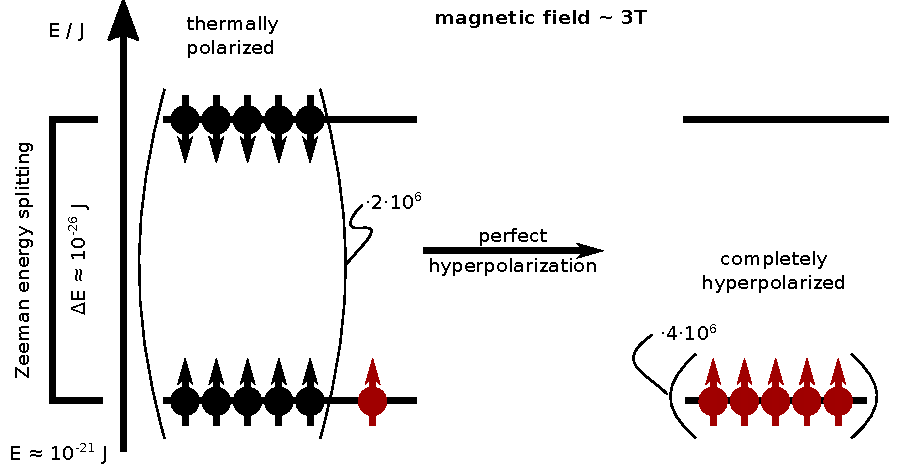
\includegraphics[width=0.9\textwidth]{/figures/theory/hyperpolarizationScheme.pdf}
            \caption[Hyperpolarization scheme]{Hyperpolarization can provide the means to drop all, or at least a lot more than in the thermally polarized case, of the spins to the lower energy level. That way, the overall magnetization and thus the signal observed is a lot higher than in there thermally polarized case. The graph shows the case of perfect hyperpolarization of $^{1}$H at \SI{3}{\tesla}, which of course does not represent reality. At the fields currently used in clinical routine, only about one in 100000 spins effectively contributes to the signal.}
            \label{figure:theory:boltzmannDistribution}
        \end{figure}
        \subsection{Dynamic nuclear polarization}
        As the gyromagnetic ratio of electrons is much higher than that of any nucleus (factor of $10^{3}$ compared to protons), dynamic nuclear polarization (DNP) uses electrons at low temperatures and high fields to generate large initial electron polarization \cite{berliner_spin_1976}. The polarization is then transferred to specific nuclei by \si{\giga\hertz} microwave irradiation \cite{bajaj_dynamic_2011} that induces transitions in the spin system of nuclei and electrons that is artificially generated by the addition of free radicals which provide an unpaired electron spin that couples to the nuclear spins. The low temperatures usually required for DNP lead to a freezing of the sample and microwaves are applied to it in that frozen state. For administration to a specimen or patient, the frozen sample then needs to be quickly melted and transferred \cite{johannesson_dynamic_2009}, usually in controlled magnetic environments \cite{milani_magnetic_2015} to prevent fast relaxation. The samples can show high polarizations close to unity but are usually limited by decay during the relatively long delivery times. Efforts building faster transport mechanisms have greatly reduced these times but they stay in the range of tens of seconds.
        \subsection{Hyperpolarization of noble gases}
        Noble gases such as 3He or 129Xe can be hyperpolarized by optical pumping \cite{middleton_mr_1995,oros_hyperpolarized_2004}. To do so, usually lasers are focused onto an optical cell through which the gas flows. The hyperpolarization is induced via the polarization of electron spins. An alkali metal, often Rubidium \cite{hersman_large_2008}, serves as a receptor for the laser induced optical pumping and subsequently hyperpolarizes the nuclei of the noble gas by spin exchange interactions \cite{walker_spin-exchange_1997}. Hyperpolarized gases are primarily used in lung imaging, but other uses e.g. in liquid state NMR or MRI by gas dissolution are not precluded \cite{duhamel_xenon-129_2001}.
        \subsection{Brute force hyperpolarization}
        As equation \ref{equation:theory:polarization} indicates, there are two main factors influencing polarization: magnetic field and temperature. It is not an option to freeze the objects to be measured, as strong polarization effects occur only close to absolute zero temperatures at the magnetic fields that can currently be generated. A viable alternative is to hyperpolarize a frozen tracer at high fields, thawing it and administering it to the subject \cite{hirsch_brute-force_2015}. Here, in contrast to DNP, no free radicals are necessary to generate the HP and - depending on the relaxation constants in the field and temperature regime - no or less harmful additives than the free radicals for DNP are necessary. This makes a faster and lossless transfer of the sample to the subject possible. The high polarization generated on $^{1}$H can then be transferred to x-nuclei e.g. by passing the sample through low fields (< \SI{10}{\milli\tesla}). The transfer is driven by thermal mixing \cite{goldman_overview_2008} of the two spin species.
        \subsection{Parahydrogen induced Hyperpolarization}
            Hydrogen is a spin 1/2 particle and thus underlies the Fermi-Dirac statistics. Its angular momentum is described by the nulear angular momenta and the rotational angular momentum. Hydrogen molecules occur in one of the four spin states
            \begin{equation}
                 \begin{aligned}
                     T_+ &=\ket{1,1} & = & |\uparrow\uparrow\rangle\\
                     T_0 &= \ket{1,0} & = &\frac{1}{\sqrt{2}}\left(|\uparrow\downarrow\rangle + |\downarrow\uparrow\rangle\right)\\
                     T_- &= \ket{1,-1}& = & |\downarrow\downarrow\rangle\\
                     S &= \ket{0,0} & = &\frac{1}{\sqrt{2}}\left(|\uparrow\downarrow\rangle - |\downarrow\uparrow\rangle\right)
                 \end{aligned}
            \end{equation}
            where T indicates the triplet state with overall spin I = 1 and S the singlet state with I = 0. Parahydrogen is the singlet state of the hydrogen molecule, i.e. the antisymmetric mixed up/down state. The molecules spin states are coupled to their rotational states. At room temperature, the even and odd rotational states are almost equally occupied which in turn means that the four spin states are also almost equally occupied as thermal energy is large compared to rotational energies of the molecule \cite{green_theory_2012-1}:
            \begin{equation}
                \frac{N_{para}}{N_{ortho}} = \frac{\sum_{J=even}(2J+1)\exp\left(-\frac{J(J+1)\Theta_R}{T}\right)}{3\sum_{J=odd}\left(2J+1\right)\exp\left(-\frac{J(J+1)\Theta_R}{T}\right)}
            \end{equation}
            where J is the rotational quantum number, $\Theta_R$ is the rotational energy constant of parahydrogen \cite{noauthor_orthohydrogen_1935}. At high temperatures, the exponential terms approach 0 and the ratio converges towards $\tfrac{1}{3}$. That means that compared to the thermal energy, the rotational energies can be neglected to a good approximation at room temperature. Approaching absolute zero, the fraction of pH$_2$ rises towards the pure pH$_2$ state as the denominator approaches zero (see figure \ref{figure:theory:ph2Fraction}). At temperatures used to generate parahydrogen in this work, around \SI{21}{\kelvin}, the pH$_2$ fraction is close to 1 with about \SI{98}{\percent} parahydrogen fraction.
            The conversion of oH2 to pH$_2$ and back is forbidden quantum mechanically due to the necessary change in spin angular momentum (0 to 1) that would change the symmetry of the wavefunction (Pauli principle)\todo{discuss with Stephan}\cite{minaev_spin_1995}. Therefore, conversions are only possible if different molecules collide and their nuclei interact or if the magnetic momentum of the rotating molecule interacts with the nuclear momenta, which is both improbable and thus slow. Theoretical lifetimes in neat gas are in the range of years \cite{green_theory_2012-1}, though in reality, e.g. through interaction with vessel walls, these long lifetimes reduce to the order of days. As the transition is forbidden in both directions, to be able to generate pH$_2$ fast and in large quantities, additional interactions need to be introduced that catalyzes the conversion. Both charcoal catalysts and ironoxide have been proposed \cite{dechent_proton_nodate}. The catalyst creates field gradients on the scale of the hydrogen molecule which enables spin mixing of ortho and para states\cite{minaev_spin_1995} and thus a much faster conversion. This means that, at liquid helium temperatures which were used in this work, parahydrogen can be enriched to almost \SI{100}{\%}, a liquid nitrogen generator would enrich it to about \SI{50}{\%} \cite{zhuzhgov_low-temperature_2018}.
            As parahydrogen itself is a spin 0 particle, it is MR-invisible. Its ordered state can be used though to polarize other molecules, often referred to as substrate molecules or target molecules.
            \begin{figure}
                \centering
                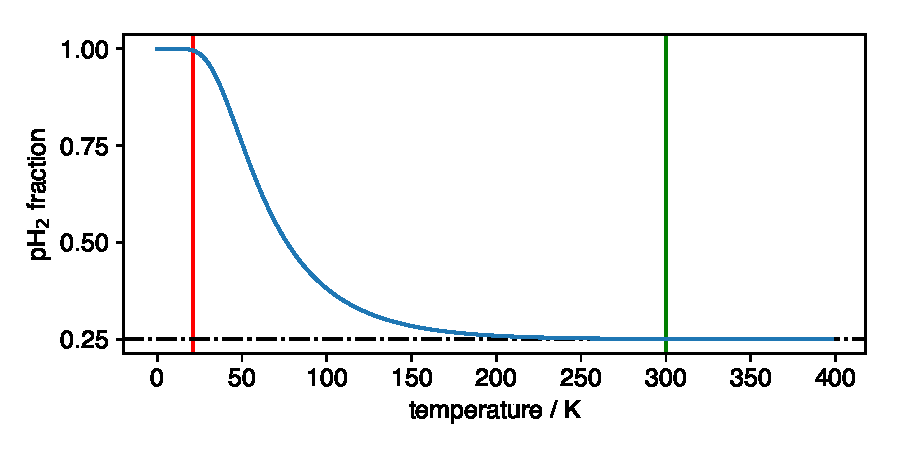
\includegraphics[width=0.9\textwidth]{/figures/theory/parahydrogenFraction.pdf}
                \caption[Parahydrogen fraction]{The equilibrium population of the para hydrogen state. The dashed line shows the high temperature limit of 3:1. The green line indicates room temperature, where the limit is almost reached. The red line indicates the temperature at which parahydrogen was generated in this work, \SI{21}{\kelvin}.}
                \label{figure:theory:ph2Fraction}
            \end{figure}
            The initial density matrix of parahydrogen can be described by
            \begin{equation}
                \sigma_0^{pH_2} = \frac{1}{4} \hat 1 - c_0(\hat{I}_1\hat{I}_2)
            \end{equation}
            with the individual spins' operators denoted by 1 and 2 \cite{green_theory_2012-1} and the constant $c_0$ scaling with the fraction of $pH_2$ in the initial gas mixture:
            \begin{equation*}
                c_0=(4f_p-1)/3.
            \end{equation*}
            The evolution of the states is then described by the evolution of the density matrix under the J couplings and chemical shifts in the target molecule and other surrounding nuclei. 
        \subsubsection{Pasadena \& PHIP}
        The first parahydrogen induced polarization (PHIP) experiments were performed at the CIT in Pasadena \cite{bowers_parahydrogen_1987-2}, and later named after it (Pasadena/Altadena). These experiments used parahydrogen to hydrogenate a molecule first and then utilized pulse sequences or field shuttling to generate observable magnetization from the parahydrogen singlet state (broken by the two distinct couplings in the molecule). Later, polarization was also transferred to nuclei other than 1H. Mostly, 13C-labeled molecules were used as recipients of the spin order and subsequent polarization. Figure \ref{fig:theory:pasadena} visualizes the hydrogenation of fumaric acid to pyruvic acid. Polarization transfer to the $^{13}$C atom with which the molecule was previously labeled would follow the hydrogenation.
        \begin{figure}
            \centering
            \includegraphics[width=0.9\textwidth]{/figures/theory/pasadena.pdf}
            \caption[Pasadena hyperpolarization]{Hydrogenation scheme used to hyperpolarize the $^{13}$C labeled fumaric acid through hydrogenation with parahydrogen to pyruvic acid.}
            \label{fig:theory:pasadena}
        \end{figure}
        To make hyperpolarization possible, the parahydrogen needs to be added to the molecule pairwise, but have to be magnetically distinct after addition \cite{eisenberg_parahydrogen-induced_1991}. That means that after the addition, the symmetry of the added hydrogen molecule must be broken to be able to transfer the spin order. This usually happens already through the asymmetry of the receptor molecule and the different couplings or chemical shifts of each added hydrogen atom of the molecule. Recently, the method has been extended and is now also used to hyperpolarize molecules that are more biologically relevant such as $^{13}$C labeled pyruvate \cite{cavallari_metabolic_2019}.
        \subsubsection{Sabre hyperpolarization}
        \label{sec:theory:HPSabre}
        The signal amplification by reversible exchange (Sabre) method was developed in 2009 \cite{adams_reversible_2009-2} for pyridine as a substrate and an Ir-based catalyst.
        In SABRE, the molecule to be hyperpolarized is not hydrogenated, but is in contact with parahydrogen via the Ir-based catalyst, $\mathrm{IrH_2(COD)(PCy_3)(MeCN)}$, often referred to as IrIMes, for a certain contact time $t_c$. The transfer of spin order can happen spontaneously at the right fields \cite{atkinson_spontaneous_2009-1} where so called level-anti-crossings (LACs, sec. \ref{sec:theory:LAC}) occur. In addition, hyperpolarized substrate can also be generated at fields far from these LACs using RF-irradiation \cite{pravdivtsev_spin_2014, knecht_quantitative_2019} and can also be enriched using selective pulse sequences \cite{knecht_re-polarization_2018-1}. The system can be described by time evolution periods in bound and unbound state, respectively, where the bound state implies non-zero couplings between pH$_2$ and at least one of the substrate spins.
            \begin{figure}
                \centering
                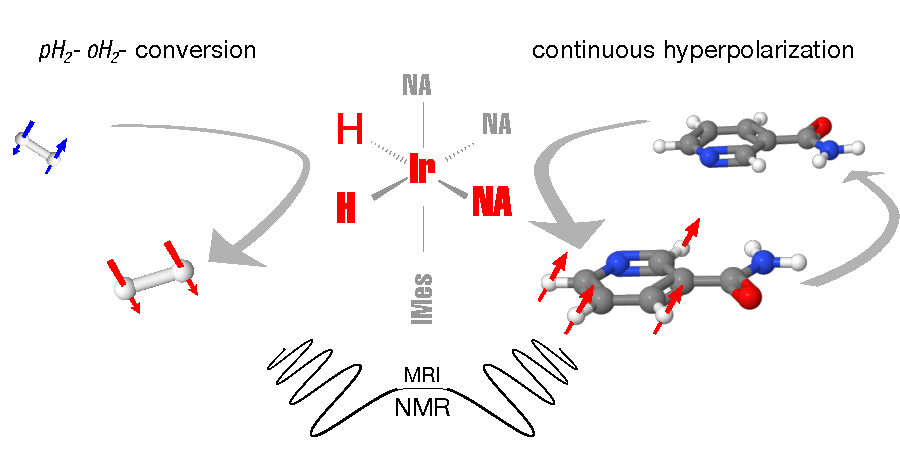
\includegraphics[width=0.9\textwidth]{/figures/theory/sabreScheme.pdf}
                \caption[Sabre scheme]{The mechanism of SABRE using nicotinamide as an exemplary molecule. On the left, parahydrogen is converted to its ortho state. On the right, nicotinamide is hyperpolarized. Centrally, a simplified chemical structure of the catalyst is shown.}
            \end{figure}
            To describe the time evolution of the bound system, the density matrix has to be evolved under the couplings present in the complex that forms when both parahydrogen and substrate are bound to, and thus coupled via, the catalyst \cite{cowley_iridium_2011-1}. The necessary Hamiltonian is formed by the Zeeman term and all the relevant couplings:
            \begin{equation}
                \begin{aligned}
                    \mathcal{H}& = \mathcal{H}_z + \mathcal{H}_J \\
                        & =\-2\pi\gamma B_0 \sum_n{(1-\delta_n)\hat{I}_{nz}} + \sum_{n<m} -2\pi J_{nm}(\hat{I}_{nx}\hat{I}_{mx} + \hat{I}_{nx}\hat{I}_{mx}+ \hat{I}_{ny}\hat{I}_{my} + \hat{I}_{nx}\hat{I}_{mx})
                \end{aligned}
            \end{equation}
            The binding time that depends on temperature and diffusion constants of the solvent has a strong influence on the effectiveness of the polarization process. Using the time evolution of the Hamiltonian, optimal time values can be found for different settings.
            Hyperpolarization occurs at different points in the system: The substrate itself is hyperpolarized, in both its bound and free form, i.e. after detaching from the catalyst. These forms can be differentiated by their different chemical shifts. At common concentrations, where a excess of target substrate is present, the free form will exceed the bound form drastically. Additionally, the hydrogen will be in a ortho state and hyperpolarized after polarization has been transferred to the target molecule. 
        \subsection{Level anti crossings}
        \label{sec:theory:LAC}
        The effect the SABRE method is based on, can be explained by observing the populations of two energy levels magnetic fields around a point of degeneracy. When coupling between the nuclei leads to a deviation from the pure Zeeman energy levels, the so called level anti crossings (LACs) or avoided crossings. In the uncoupled case, two energy levels  can cross at a certain magnetic field strength, i.e. the two states would have the same energy at that point \cite{ivanov_role_2014-2,pravdivtsev_spin_2014}:
        \begin{equation}
            E_0 = E_1 \mathrm{~~\rightarrow~~} \bra{0}H\ket{0} = \bra{1}H\ket{1}
        \end{equation}
        If the nuclei are coupled though, the crossing is avoided and there is a defined energy difference between the nuclei's states in the central region of the avoided crossing; the size is determined by the strength of the coupling. Figure \ref{figure:theory:LAC} shows such a crossing for two states crossing in the uncoupled case (red stripes), but avoiding that crossing in the coupled case by $J_{12}$. The Hamiltonian of the system is
        \begin{equation}
            H = \left [
                \begin{array}{ll}
                    E_{1} & W_{12}\\
                    W_{21} & E_2
                \end{array}
            \right ]
        \end{equation} 
        where $W_{12}$ is the coupling between the energy levels $E_1$ and $E_2$ which leads to new eigenenergies
        \begin{align*}
            E_+ &= \frac{1}{2} \left[(E_0+ E_1) + \sqrt{(E_0-E_1)^2+4|W_{12}|^2}\right]\\
            E_- &= \frac{1}{2} \left[(E_0+ E_1) - \sqrt{(E_0-E_1)^2+4|W_{12}|^2}\right]
        \end{align*}
        which, for $W_{12}=0$ gives the Eigenstates of the uncoupled system, $E_1$ and $E_2$. The corresponding new Eigenstates are 
        \begin{equation*}
            \ket{+} = \cos\frac{{\theta}}{2}\exp{i\phi}\ket{0} + \sin{\frac{\theta}{2}}\exp{i\phi}\ket{1}\\
        \end{equation*}
        \begin{equation*}
            \ket{-} = -\sin{\frac{\theta}{2}}\exp{i\phi}\ket{0} + \sin{\frac{\theta}{2}}\exp{i\phi}\ket{1}
        \end{equation*}
            \begin{figure}
                \centering
                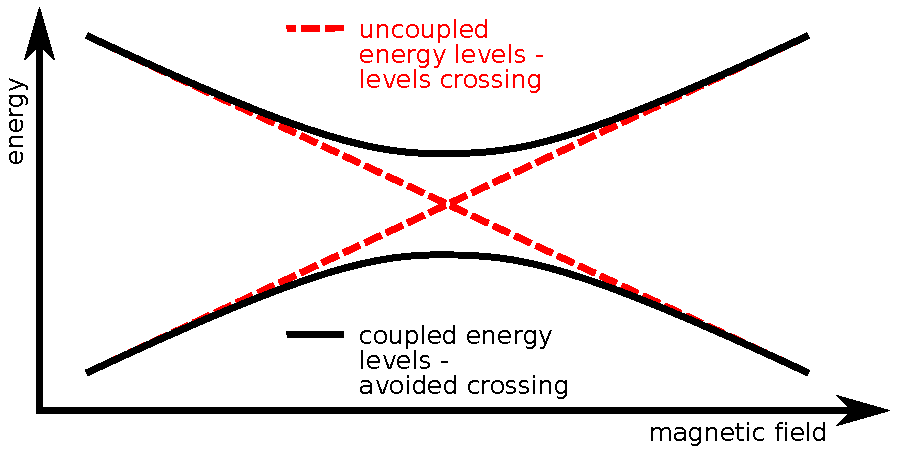
\includegraphics[width=0.9 \textwidth]{/figures/theory/LACs.pdf}
                \caption[Level anti crossings]{A generic example of level anti crossings. In red, the uncoupled states can be seen while in black, the energy states in the presence of coupling are shown.}
                \label{figure:theory:LAC}
            \end{figure}
            This means that the coupling leads to a mixing of the states if the magnetic field, which determines the energy difference between $E_2$ and $E_1$, is in the region of the LAC. Effectively, the coupling thus changes the occupational numbers of the uncoupled states over time. See section \ref{sec:theory:HPSabre} for how this effect can be used to hyperpolarize samples.
        \section{Hardware}
            As hardware plays an important role in this work, I also want to provide a bit of theoretical insight into some of the technologies used in this work.
            \subsection{Field generation}
                The magnetic fields are generated by either current flown conductors or superconductors with exception of a few cases where permanent magnets are used. Both normal and superconductors have ad- and disadvantages and are chosen according to requirements (see \ref{chap:MaterialsAndMethods}). Magnetic field is generated according to the fourth Maxwell equation
                \begin{equation}
                    \label{equation:theory:maxwell}
                    \vec\nabla\times\vec B = \mu_0\vec j+\mu_0\epsilon_0\frac{\partial\vec E}{\partial t}
                \end{equation}
                where $\vec j$ is the electric current generating the magnetic field together with changes in the electric field \cite{b.i._bleaney__b._bleaney_electricity_nodate}. For the static field of a conductor, the current is the main mechanism of field generation and is described by the Biot-Savart-law.
            \subsubsection{Normal conductors}
                A normal conductor has the great advantage of room temperature operation, simplifying its setup and use enormously. The disadvantage is  its finite resistance. That means the conductor will heat which will limit the maximum current at which it can be safely operated.  That heating can be so large that melting of the conductor occurs or, in the less dramatic case, deformations happen due to heat expansion and/or softening of the conductor material. Usually, copper is chosen for its low electric resistance of \SI{1.72e-8}{\ohm\meter}(reducing heat generation) and at the same time high thermal conductivity \SI{380}{\watt\per\m\per\kelvin}(increasing heat dissipation) \cite{schofield_f._h._thermal_1925}.
            \subsubsection{Superconductors}
            \label{sec:theory:superconductor}
            Superconductors are a special form of conductors that show electric resistances of exactly zero below a certain critical temperature $T_c$ discovered in 1911 \cite{onnes_resistance_nodate}. Generally, superconductors need to be cooled to a few \si{\kelvin} to show this property, modern alloys so called high temperature superconductors can, under certain conditions, raise that limit to about \SI{200}{\kelvin} \cite{drozdov_conventional_2015}. Superconductors can be made of different, rather exotic materials but also more common substances such as graphene can show superconducting properties \cite{cao_unconventional_2018}. Different superconductors show different critical Temperatures and mechanical properties often restricting their use to certain fields. Microscopically, inside the superconductors, so called cooper pairs are forming \cite{bardeen_theory_1957}. These pairs of two electrons travel resistance free through phonon coupling, i.e. the deformation of the surrounding lattice caused by one electron distribution and the related energy loss is regained \SI{100}{\percent} by a second electron. That way, completely lossless movement of electrons is possible in the compound.
            \subsection{Magnetic susceptibility and shielding}
                The magnetic field generated by a current flow or a changing electric field is described by the magnetic field strength $\mat H$ which describes the magnetic field with no material present. The actually relevant size for experimental purposes is the magnetic flux density $B$ which adds to the magnetic field strength the magnetization $M$ of materials exposed to the magnetic field strength $H$.
                \begin{equation}
                    \vec{B} = \mu \vec{H} = \mu_0 \mu_r \vec{H} = \mu_0(1+\chi) \vec{H}
                \end{equation}
                where $\chi$ is the magnetic susceptibility \cite{schenck_role_1996}, the quantity mostly mentioned in NMR and MRI. Usually, $B$ is the quantity intended when talking about magnetic fields.
                In many cases, as for example for air, $B$ and $H$ are almost the same as the relative permeability \cite{kriz_magnetic_1996} $\mu_r$ is only 0.35 ppm \cite{cullity_introduction_2008}. For water, it is already about a factor 10 higher, i.e. $\mu_r$ = 2~ppm . 
                This means that, where susceptibility changes occur in materials, magnetization and thus magnetic field's change. These changes cause field inhomogeneities posing a problem for NMR and MRI where a more homogeneous field ($B_0$) is always preferred. Materials are grouped by their susceptibilities \cite{b.i._bleaney__b._bleaney_electricity_nodate}:
                Substances with a large, positive $\chi$ are called ferromagnetic, they are magnetized in the direction of the external field and the magnetization can surpass the field strength of the external field. External field and magnetization aren't usually linearly correlated for ferromagnets, when all magnetic moments in the material are aligned a plateau is reached. Usually, these materials follow a magnetization hysteresis when the external field changes value and sign. Furthermore, ferromagnets do not necessarily return to their unmagnetized state if H returns to 0 (remanence).
                Paramagnetic and diamegnetic substances show a much smaller magnetization, where paramagnetic substances' nuclear momenta, as ferromagnetic ones, align parallel to the magnetic field ($\chi>0$) and diamagnetic antiparallel ($\chi$ < 0).
                Shielding of external magnetic fields can make use of the fact that the high susceptibility of some materials leads to a bundling of magnetic field lines, i.e. a volume surrounded by that material can have a strongly reduced magnetic flux density and thus a lower magnetic field \cite{mager_magnetic_1970}.
            \subsection{Oscillating circuit}
                A coil for usage in NMR or MRI usually consists of oscillatory circuits made up of a capacitor of capacitance $C$ and an inductance $L$. Inside a oscillatory circuit, energy can be stored in the forms of electric field and electric current. The two forms of energy are constantly converted into each other, i.e. the capacitor is charged by the current coming from the coil and in turn generates a phase shifted countering current. The frequency of this conversion can be calculated considering the following differential equations:
                \begin{equation}
                    \begin{aligned}
                        -L\frac{dI}{dt} &= \frac{Q}{C} \\
                        L\frac{d^2I}{dt^2} + \frac{I}{C} &= 0
                    \end{aligned}
                \end{equation}
                as the voltages of coil - that is proportional to the change in current according to Faraday's law - and the capacitor - that depends on capacitance and charge - need to be equal at all times. The solution of this simplified case resulting in a ordinary second order differential equation with no linear term is simply a undampened oscillation:
                \begin{equation}
                    I(t) =  A \cdot \cos(\omega t) + \phi 
                \end{equation}
                where $f= \frac{1}{\omega} = \frac{1}{2\pi\sqrt{LC}}$ which means that by changing capacitance and inductance in a resonant circuit, the resulting resonance frequency can be changed \cite{rao_electronic_2011}. Moreover, capacitance and inductance sizes can be adapted in opposite directions depending on the purpose of operation.
                Of course, in realistic cases, the oscillation is dampened by ohmic resistance of the components and radiation losses.
            \subsection{Birdcage coils}
            Commercially available volume resonators are often manufactured in the birdcage design. The advantage of that design is the alignment of the coil's open and accessible axis with the magnetic field, meaning the coil can be accessed and loaded while installed in the scanner bore. Exchanging or repositioning samples is possible without removing the coil. The design is based on an array of individual resonant circuits, mostly in a bent, rectangular shape called leg where one side of the leg is a conductor shared by the neighboring legs The rotating magnetization induces a current in those legs, the currents in neighboring legs are phase shifted according to the overall number of legs $\phi_{mag} = 360\si{\degree}/n_R$. As the total phase shift over the resonator must be a multiple of 2$\pi$, if all legs' impedances are the same, the coil can be driven and read out at two points only - generating the above mentioned pahse shift by itself. Birdcage coils are mostly chosen for transmission, in small animal scanners, in contrast to human scanners, where the distances are often too large, they're also used as receive coils in rodents where the diameters of the specimen are relatively small.
            \subsection{Saddle coil}
            \label{sec:theory:saddleCoils}
            The saddle coil used for RF-excitation of the sample is designed based on the publication by Hoult, \cite{hoult_signal--noise_1976}. It derives that the field generated by a saddle coil is given by
            \begin{equation}
                B_{xy} = \frac{\sqrt 3 \mu\mu_0}{\pi}\left(\frac{ag}{(a^2+g^2)^{3/2}}+\frac{g}{a(a^2+g^2)^{1/2}}\right)
            \end{equation}
            where a is the radius of the coil and g is half the height. Using these calculations, an optimum field homogeneity is reached when the opening angle of the coil is \SI{120}{\degree} and the length is equal to the diameter of the coil.
            \subsection{Nyquist theorem}
            Especially in the low field spectrometer case, where no frequency mixing is performed as is usually the case at the MRI's much higher frequencies, one had to keep in mind sampling theorems to ensure a proper signal coverage. A signal needs to be sampled at a minimum sampling frequency \cite{shannon_mathematical_1948}
                \begin{equation}
                    \label{equation:theory:nyquist}
                    f_{s} = 2 f_{sig}
                \end{equation}
                if signals with a maximum frequency of $f_{sig}$ are expected. If the sampling frequency is lower than that, aliasing effects will occur. Specifically, fold ins in the Fourier transform will show up. Fold ins are higher frequency signal sources $f_{high}$ that show up at frequencies smaller than the minimum sampling frequency from equation \ref{equation:theory:nyquist}. Frequencies are mapped back to
                \begin{equation}
                    f_{fi}(n) = f_{sig,high} - n * f_s
                \end{equation}
                where $|n\cdot f_s| < |f_{sig,high}| < |n+1 \cdot f_s|$. Note that the signal would show up at all frequencies $f_{fi}(n)$ but usually is visible only once due to the previously chosen readout frequency band.
                Another option would be to limit the bandwidth towards the lower end by a high pass filter and use this a priori knowledge to prevent the aliasing.
            \subsection{Operational amplifiers}
                Operational amplifiers have been used to amplify the signal of the fluxgate magnetic field sensor. Amplification is necessary because of the large output range of $\pm$ \SI{10}{\volt} in combination with the high resolution in the low field regime. Operational amplifiers are a rather complex network of transistors that show a behavior similar to what is described in the following. The ideal operational amplifier amplifies the incoming signal to infinity on the positive input, to $-\infty$ on the negative input and has an infinite input impedance as well. This is not true in practice, but very high voltages (limited by the supply voltage) are produced at the output if a small voltage is applied to either of the inputs. With the gain $A_{opa}$, the output voltage is thus described by
                \begin{equation}
                        \label{equation:theory:OPAvoltage}
                    U_{out} = A_{opa}(V_+ - V_-)
                \end{equation}
                That is why operational amplifiers need to be driven in some kind of feedback mode (figure \ref{figure:theory:opAmp}) as otherwise even very small voltage differences on the input cause a saturation of the output. In this mode, the output is fed back to one of the inputs, most of the time via resistors, to generate a defined output voltage that depends on the input voltage of the complete setup, $U_{in}$. The so called inverting opamp that was used in this work, is shown in figure \ref{figure:theory:opAmp} and will be described in more detail now.
                \begin{figure}
                    \includegraphics[width=0.9\textwidth]{/figures/theory/opAmp.pdf}
                    \caption[Operational amplifier]{An operational amplifier in an inverting setup. The amplification of the input voltage $U_{in}$ is directly given by the ratio of the resistors, $R_2/R_1$.}
                    \label{figure:theory:opAmp}
                \end{figure}
                By connecting the output to the negative input, a loop is formed in which the voltages add to zero. This tells us that
                \begin{equation*}
                    U_{opa} = U_{out} - U_- = U_{R_2}
                \end{equation*}
                Additionally, as, as soon as the negative input starts to differ from the positive one, the output reacts and drives it back. That way, there is a virtual ground on the negative input (marked with a red dot in figure \ref{figure:theory:opAmp}).
                This can also be shown by calculating the voltage $U_-$:
                \begin{equation}
                    U_- = U_{in} + U_{R_1} = U_{R_2} + U_{out}
                \end{equation}
                which, considering $R_1$ and $R_2$ are a voltage divider due to the lack of current trough the opamp, this can be written as
                \begin{equation}
                    U_{-} = U_{out} \frac{R_1}{R_1+R_2} + U_{in} \frac{R_2}{R_1+R_2}
                \end{equation}
                and, if combined with equation \ref{equation:theory:OPAvoltage}, gives the output voltage
                \begin{equation}
                    U_{out} = -U_{in} \frac{A_{opa}R_2}{R_1+R_2 + A_{opa}R_1}
                \end{equation}
                which, for large $A_{opa}$ present in all operational amplifiers simplifies to the resistor ratio.
                \begin{equation}
                    U_{out} = -U_{in}\frac{R_2}{R_1}
                \end{equation}
                This also makes sense phenomenologically: with this setup, $U_{+}$ and $U_{-}$ are kept at the same level, i.e. the negative input acts as a virtual ground, as the output is fed back to the negative input and any perturbance that causes a differential voltage between the two inputs will regulate itself by applying a corresponding voltage to the negative input until equilibrium is restored \cite{huijsing_operational_2017-1}.
                This is especially helpful as the accuracy of the resistors is the limiting factor of the amplification's accuracy, i.e. by choosing the resistors carefully, the amplification can be set very accurately.
            \subsection{Frequency filters}
            For reducing noise when interested in certain regions of the frequency spectrum only, frequency filters can be used. They differ in the steepness of the cutoff frequency, so-called order, and the transmission efficiency (no Filter is completely lossless at the unblocked frequencies). The easiest frequency filter is just a combination of a capacitor and a resistor or a inductance and a resistor as shown in figure \ref{figure:theory:frequencyFilter}. Using the impedances of inductance and capacitor
                \begin{equation*}
                    Z_C = -i\frac{1}{\omega C}
                \end{equation*}
                \begin{equation*}
                    Z_L = {i\omega L}
                \end{equation*} 
                The output voltage $U_o$can then be described as a function of input voltage $U_{i}$ and these two impedances:
                \begin{equation}
                    U_o = \frac{Z_c}{Z_R + Z_C} U_i
                \end{equation}
                with the signal frequency $\omega$. The cutoff frequency of the filter $f_0$ can then be described for both the RC-filter by
                \begin{equation}
                    f_0^{RC} = \frac{1}{2\pi R C}
                \end{equation}
                and the RL-filters:
                \begin{equation}
                    f_0^{RL} = \frac{R}{2\pi L}
                \end{equation}
                where the arrangement of the components defines whether it is a low or a high pass filter. These filters are the simplest form of frequency filters of first order and show a boundary drop of \SI{20}{\deci\bel} per frequency decade. Higher order filters can be used where more sharply defined cutoff frequencies are necessary but usually come with drawbacks in the linearity of the transmit band especially close to the cutoff frequency (ripple). These can be constructed by combining multiple frequency filters serially or by designing more complex filters such as the Chebyshev filter, a LC filter with n stages. Figure \ref{figure:theory:frequencyFilter} demonstrates the effect of first and second order filters on the signal at different frequencies.
            \begin{figure}
                \centering
                \includegraphics[width=0.9\textwidth]{/figures/theory/frequencyFilters.pdf}
                \caption[Frequency filters]{Transfer function over frequency for the different types of filters mentioned in the text. Cutoff frequencies are shown for the filters. At the frequency value of 10, a first order high and low pass filter are shown for the same cutoff frequency (i.e. same L/C and R values) in purple colors. Further to the right, a shifted first order filter (C/L * 10) and a second order filter are shown in shades of red.}
                \label{figure:theory:frequencyFilter}
            \end{figure}
            \subsection{Flow and flow resistance}
                Pressure differences above liquids or in gases create flow from high to low pressure volumes. These flows are important in the setups used here and will be shortly described as a function of the pressure creating them under simplified conditions. The flow is described by the Navier Stokes equations \cite{sochi_flow_2013}.
                Flowing speeds are generally limited by the flow resistance. This resistance is easily described if the flow is through a tube and can be considered laminar. Generally, the volume flow rate Q is given by the Hagen-Poiseuille equation:
                \begin{equation}
                    Q=\frac{p_2-p_1}{R}
                \end{equation}
                where R is the Reynolds number. Using an electrical circuit as a similarly described system, the Reynolds number would correspond to electrical resistance and the pressure difference would be a voltage equivalent. The Reynolds number generally depends on $\eta$, the viscosity of the fluid and the flow resistance of the connecting vessel. For example, for a solid tube of radius r and length l, the Reynolds number is given by \cite{jeffrey_particle_1965}
                \begin{equation}
                    R=\frac{8\eta l}{\pi r^4}
                \end{equation}
                Because of the much lower viscosity of gases that stems from their lower density, gas flow is generally higher than fluid flow at otherwise unchanged conditions.
